\documentclass[12pt, letterpaper]{report}
\usepackage{graphicx}
\usepackage{hyperref}
\usepackage{amssymb}
\usepackage{amsmath}
\usepackage{float}
\usepackage{mathtools}
\usepackage{enumitem}
\usepackage[margin=1in]{geometry}
\usepackage[figurename=Figura]{caption}
\title{Fuentes de Campo magnético}
\author{Juan Pablo Guerrero Escudero}
\date{26 may, 2024}
\begin{document}
\maketitle
\subsubsection*{Campo magnético por una carga en movimiento}
El campo magnético $\vec{B}$ es generado por una partícula en movimiento, y su 
dirección siempre es perpendicular al plano formado entre los vectores $\vec{v}$ y $\vec{r}$, que 
es el vector de desplazamiento desde el punto de la carga en movimiento, hasta el punto donde se 
busca encontrar el campo magnético. En la línea donde corre con velocidad constante la carga en movimiento, 
el campo magnético es 0. Además, se puede encontrar la dirección de las líneas de campo magnético con la regla de la mano 
derecha, al apuntar el pulgar hacia la dirección de $\vec{v}$, y al cerrar los dedos estos nos dicen la dirección de las líneas 
de campo magnético. En el siguiente diagrama se ilustra de mejor manera: 
\begin{figure}[H]
    \centering
    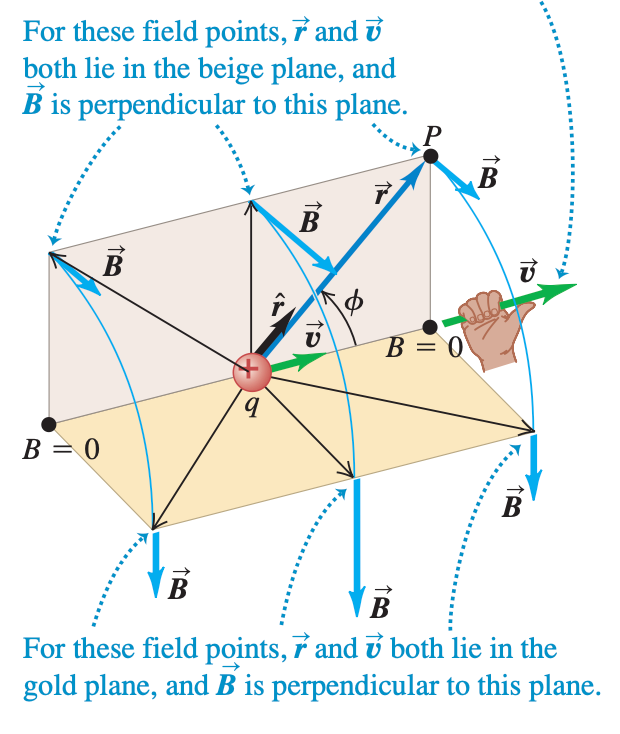
\includegraphics[height = 8cm]{2024-05-26_DiagramaCampoMagnetico_1.png}
    \caption{Diagrama campo magnético generado por una carga positiva en movimiento}
\end{figure}
La fórmula experimental para encontrar el campo mangético generado por una carga positiva en un punto $P$ es: 
\begin{align}
\vec{B} &= \frac{\mu_0}{4\pi}(\frac{q \vec{v} \times \hat{r}}{r^2})
\label{eq:eq1}
\intertext{Y para encontrar su magnitud}
B &= \frac{\mu_0}{4\pi}(\frac{|q|\ast v \ast \sin{\phi}}{r^2})
\label{eq:eq2}
\end{align}
En la fórmula anterior, $\phi$ representa el ángulo de separación entre $\vec{v}$ y $\hat{r}$, $K_m = \frac{\mu_0}{4\pi} = 10^{-7} T m/A$, $\mu_0 = 4\pi \times 10^{-7} T \cdot m / A$
y el campo magnético se 
maximiza cuando $\phi = 90$ porque $\sin(90) = 1$, es decir, en el plano perpendicular al plano de $\vec{v}$ y $\hat{r}$. Por último, 
si la carga es negativa, la dirección de $\vec{B}$ es opuesta a la dirección que iría siendo carga positiva. \\
\subsubsection*{Campo magnético por una línea de corriente}
Ahora, si tenemos una corriente, el campo magnético total es la suma vectorial de cada carga dentro del conductor, o sea una suma de cargas pequeñas. Por lo tanto 
podemos usar diferenciales para ésto. Calculamos el campo magnético producido por un $d\vec{l}$ o una parte pequeña del conductor. Su volumen es $A \ast dl$ donde $A$ es 
el área cross-sectional de la figura. Ahora, las cargas en movimiento equivalen a un $dQ$, y por lo tanto obtenemos la Ley de Biot-Savart, que dice: 
\begin{align}
d\vec{B} &= \frac{\mu_0\ast I}{4\pi}(\frac{d\vec{l} \times \hat{r}}{r^2}) 
\label{eq:eq3}
\intertext{Y su magnitud se calcula}
dB &= \frac{\mu_0\ast I}{4\pi}(\frac{dl\sin{\phi}}{r^2})
\label{eq:eq4}
\end{align}
A continuación se muestra un diagrama general de la situación cuando se tiene un campo magnético generado por una línea de corriente: 
\begin{figure}[H]
    \centering
    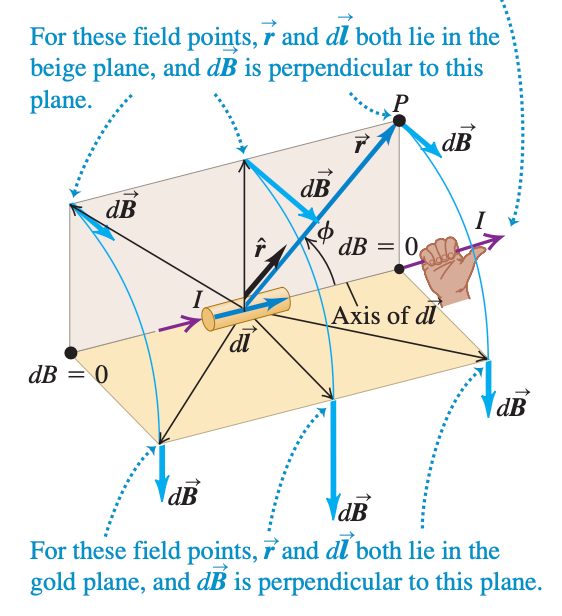
\includegraphics[height = 8cm]{2024-05-26_DiagramaCampoMagnetico_2.png}
    \caption{Diagrama campo magnético generado por una línea de corriente}
\end{figure}
En la ecuación anterior, el campo magnético es perpendicular al plano formado por $d\vec{l}$ y $\hat{r}$, donde $d\vec{l}$ tiene la misma dirección que 
la corriente en el conductor. Las fórmulas \ref{eq:eq3} y \ref{eq:eq4} se llaman Ley de Biot-Savart, y se puede 
usar para encontrar el campo magnético $\vec{B}$ en cualquier punto en el espacio debido a la corriente en un circuito. Para encontrar el campo magnético total 
$\vec{B}$, integramos todos los segmentos $d\vec{l}$, es decir $\vec{B} = \frac{\mu_0}{4\pi}(\int \frac{I\ast d\vec{l} \times \hat{r}}{r^2})$. \\

Si buscamos obtener el campo magnético en un punto P por un conductor delgado con corriente, usamos la siguiente fórmula: 
\begin{align}
\vec{B} &= \frac{\mu_0 I}{4\pi a}(\cos{\theta_1} - cos{\theta_2}) \hat{k}
\label{eq:eq5}
\end{align}
En donde $a$ es la distancia perpendicular desde el conductor hasta el punto $P$, y $\theta_1$ es el ángulo entre el conductor y el vector $\hat{r}$ en el punto 
inicial $P_i$ y $\theta_2$ es el ángulo entre el conductor y el punto final $P_f$.
Después, para encontrar el campo magnético en una línea de carga infinita, usamos la fórmula 
\begin{align}
\vec{B} = \frac{\mu_0 I}{2\pi r}
\label{eq:eq6}
\end{align}
Y esa fórmula sirve para encontrar el campo magnético en todos los puntos de un círculo de radio $r$ alrededor de un conductor 
recto infinito. 
\end{document}